\documentclass[conference]{IEEEtran}
\usepackage{graphicx,booktabs,amsmath,amssymb,url,xcolor,multirow}
\usepackage[hidelinks]{hyperref}
\graphicspath{{figures/}}
\newcommand{\repo}{\url{https://github.com/<your-username>/GenAI_Assignment1}}
\newcommand{\video}{\url{https://youtu.be/<video-id>}}

\begin{document}
\title{From Universal to Mixture-of-Experts Image Restoration, and Style-Conditioned Face-to-Sketch Synthesis:\\ Design, Evaluation and Deployment of Four Generative Models}
\author{\IEEEauthorblockN{<Your Name>}\IEEEauthorblockA{<Roll number> -- Generative AI, Assignment 1\\Code: \repo\quad Demo: \video}}
\maketitle

\begin{abstract}
We build and deploy four related generative systems. On the Oxford-IIIT Pet dataset with runtime-generated salt-and-pepper noise, Gaussian blur and rectangular occlusion, we compare (i) a single universal denoising autoencoder (UDAE), (ii) a corruption classifier that hard-routes inputs to three specialist autoencoders with an identity bypass for clean images, and (iii) a jointly fine-tuned soft mixture-of-experts (MoE) whose gate is initialised from the classifier. On FS2K we train (iv) a pix2pix-style conditional GAN whose U-Net generator and PatchGAN discriminator are both conditioned on a learned sketch-style embedding. Every model is tuned with Optuna, tracked with MLflow, exported to ONNX (verified against PyTorch to $<10^{-6}$ max absolute error), and served by a FastAPI + React application started with one Docker Compose command. \textbf{RESULTS-SUMMARY}
\end{abstract}

\section{Introduction}
Real images are degraded in heterogeneous ways, and a single restoration network must trade capacity between incompatible inverse problems: removing impulse noise requires discarding isolated outliers, de-blurring requires amplifying high frequencies, and inpainting requires hallucinating plausible content. We study three ways of organising this capacity, a shared model, hard specialisation, and soft specialisation, under one controlled corruption protocol, and complement them with a paired image-to-image GAN. The emphasis is on evidence: each design decision is backed by an ablation, an Optuna study, or a cited prior result.

\section{Related Work}
Denoising autoencoders learn robust representations by reconstructing clean inputs from corrupted ones~\cite{vincent2008}; convolutional encoder-decoders with symmetric skips are strong restorers~\cite{mao2016}, but unrestricted skips can bypass the bottleneck, which the assignment forbids. Combining an L1 term with SSIM produces sharper, perceptually better restorations than L2 alone~\cite{zhao2017}. Mixture-of-experts models route inputs to specialised sub-networks through a learned gate~\cite{jacobs1991}; sparsely-gated MoEs add load-balancing terms to prevent the gate from collapsing onto a few experts~\cite{shazeer2017,fedus2022}, which motivates our balance regulariser. Conditional GANs for paired translation (pix2pix) combine an adversarial PatchGAN loss with an L1 reconstruction term weighted by $\lambda=100$~\cite{isola2017}; class-conditioning through learned embeddings follows~\cite{mirza2014,miyato2018}. FS2K~\cite{fan2022} provides 2{,}104 photo--sketch pairs in three styles. Hyper-parameters are optimised with the TPE sampler and median pruning of Optuna~\cite{akiba2019}.

\section{Data and Corruption Protocol (Tasks 1--3)}
The official Oxford-IIIT Pet \emph{trainval} split (3{,}680 images) is divided 80/20 with seed 42 into 2{,}944 training and 736 validation images; the 3{,}669-image \emph{test} split is only touched by the final evaluation scripts. Images are converted to RGB and resized to $128\times128$ (bicubic).
\textbf{Runtime corruption.} Corruption happens inside the DataLoader's collate function, so every time an image is loaded a new condition and severity are drawn and nothing is written to disk. Task~1 draws each image's condition uniformly from \{clean, salt-and-pepper, blur, occlusion\}; Tasks~2--3 build exactly class-balanced batches. Salt-and-pepper replaces a fraction $p\sim\mathcal U(0.02,0.15)$ of pixels by black or white (50/50); blur uses $k\in\{3,5,7\}$, $\sigma\sim\mathcal U(0.5,2.5)$; occlusion inserts 1--3 non-overlapping black rectangles jointly covering $\mathcal U(10\%,35\%)$ of the image (Dirichlet area split, log-uniform aspect ratio in $[\frac12,2]$).
\textbf{Deterministic validation/test.} A validation manifest stores one fixed corruption (type, parameters, rectangle coordinates, seed) per validation image. The test manifest stores, for every test image, the clean input plus three corruptions at three fixed severities ($p\in\{0.03,0.08,0.15\}$; $(k,\sigma)\in\{(3,0.7),(5,1.5),(7,2.5)\}$; 1/2/3 rectangles covering $\approx$10/20/35\%), i.e.\ 36{,}690 test cases. The corruption code is pure NumPy and is imported unchanged by the web backend, so the app reproduces the exact test conditions. Unit tests check every range, the 50/50 salt/pepper split, occlusion coverage, determinism, and that our separable blur matches \texttt{torchvision} to $10^{-5}$.
\textbf{Metrics.} PSNR (capped at 50\,dB: an identity output on a clean input would otherwise give $\approx$100\,dB and dominate averages), SSIM (11$\times$11 Gaussian window) and L1, always against the clean target.

\section{Task 1: Universal Denoising Autoencoder}
\subsection{Architecture}
Fig.~\ref{fig:t1arch}: three stride-2 convolutional stages (channels $b,2b,4b$) reduce $128^2$ to $16^2$; a $1\times1$ convolution produces a $16\times16\times c$ latent ($c\in\{4,8,16,32\}$, i.e.\ 12--48$\times$ fewer values than the 49{,}152-value input). A mirrored decoder with transposed convolutions and a sigmoid output reconstructs the RGB image. There are \emph{no} skip connections, so all information passes through the bottleneck. Dropout2d is applied in the encoder and at the latent.
\begin{figure}[t]\centering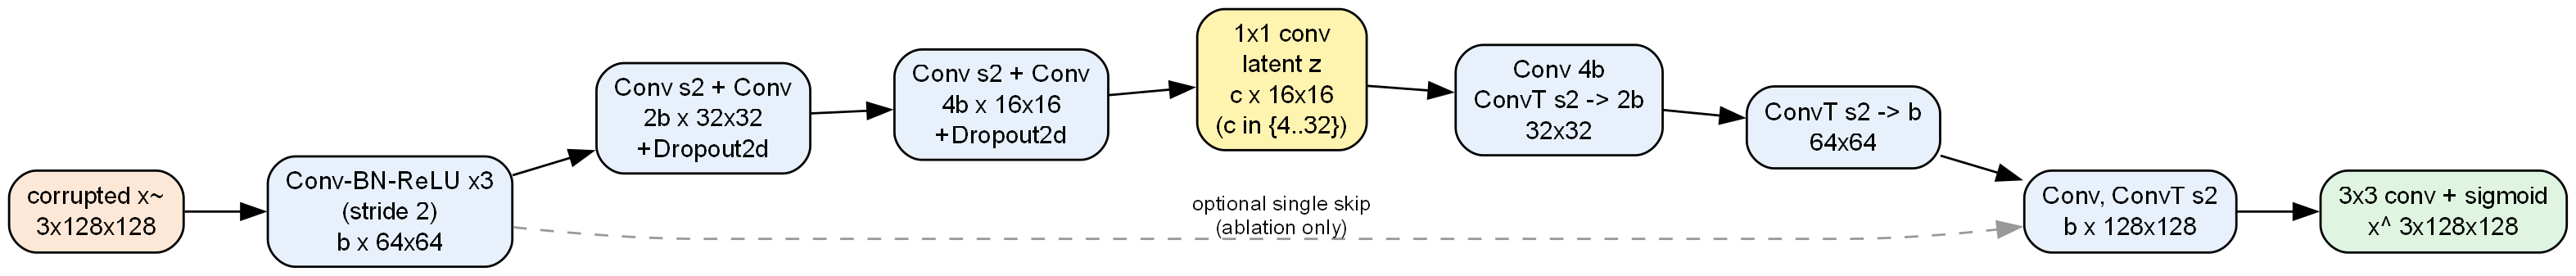
\includegraphics[width=\linewidth]{t1_udae.png}\caption{Universal DAE. The dashed skip exists only in the ablation.}\label{fig:t1arch}\end{figure}
\subsection{Loss and Optuna search}
$\mathcal L_{UDAE}=\alpha\,\mathcal L_{1}(x,\hat x)+(1-\alpha)(1-\mathrm{SSIM}(x,\hat x))$, with SSIM computed in fp32 because it was numerically unstable under mixed precision. Optuna (TPE, seed 42, median pruner after 2 epochs, 16 trials $\times$ 6 epochs) searched lr $\in[10^{-4},3\cdot10^{-3}]$ (log), batch $\in\{16,32,64\}$, latent channels $\in\{4,8,16,32\}$, base channels $\in\{16,32,48,64\}$, dropout $\in[0,0.3]$ and $\alpha\in[0.5,0.95]$; the first trial was the suggested starting point ($\alpha=0.8$). \emph{Key design choice:} the objective is validation $\mathcal L_1+(1-\mathrm{SSIM})$ with \emph{fixed} equal weights. Scoring each trial with its own $\alpha$-weighted loss would make trials incomparable and bias the search towards whichever $\alpha$ makes its own loss numerically smallest. \textbf{T1-OPTUNA} The best configuration was retrained for 40 epochs (AdamW, one-cycle LR, AMP).
\subsection{Results}
egin{table}[t]\centering\caption{Task 1 universal DAE on the official test set (3{,}669 images per condition). PSNR in dB, capped at 50.}\label{tab:t1}\setlength{	abcolsep}{4pt}
egin{tabular}{llrrrr}	oprule
Input & Sev. & PSNR$_{in}$ & PSNR$_{out}$ & SSIM$_{in}$ & SSIM$_{out}$\\midrule
Clean & none & 50.00 & 23.29 & 1.000 & 0.849 \\
S\&P & low & 20.13 & 23.27 & 0.602 & 0.846 \\
S\&P & medium & 15.87 & 23.20 & 0.340 & 0.837 \\
S\&P & high & 13.14 & 23.00 & 0.204 & 0.819 \\
Blur & low & 32.34 & 23.37 & 0.944 & 0.846 \\
Blur & medium & 26.77 & 23.02 & 0.806 & 0.816 \\
Blur & high & 24.35 & 21.92 & 0.692 & 0.711 \\
Occl. & low & 16.70 & 21.59 & 0.862 & 0.796 \\
Occl. & medium & 13.27 & 20.38 & 0.726 & 0.743 \\
Occl. & high & 10.75 & 18.90 & 0.536 & 0.663 \\
ottomrule\end{tabular}\end{table}

\textbf{T1-RESULTS}

\section{Task 2: Classifier and Hard-Routed Specialists}
A VGG-style CNN (four double-conv blocks, global average pooling, dropout, linear head) predicts \{clean, s\&p, blur, occlusion\}; cross-entropy is minimised on exactly class-balanced batches. Optuna (12 trials $\times$ 5 epochs, objective: validation macro-F1) tuned lr, batch, channel configuration (small/medium/wide), dropout and weight decay. Three specialists with the Task~1 architecture are trained only on their own corruption. To keep the search affordable we ran \emph{one shared} Optuna study (10 trials): each trial trains all three specialists for 4 epochs and is scored by the mean of their validation objectives; pruning acts on the running mean after each specialist. The selected configuration then trains three independent specialists for 30 epochs. At inference (Fig.~\ref{fig:t2arch}) the arg-max class selects one specialist, and clean inputs take an identity bypass.
\begin{figure}[t]\centering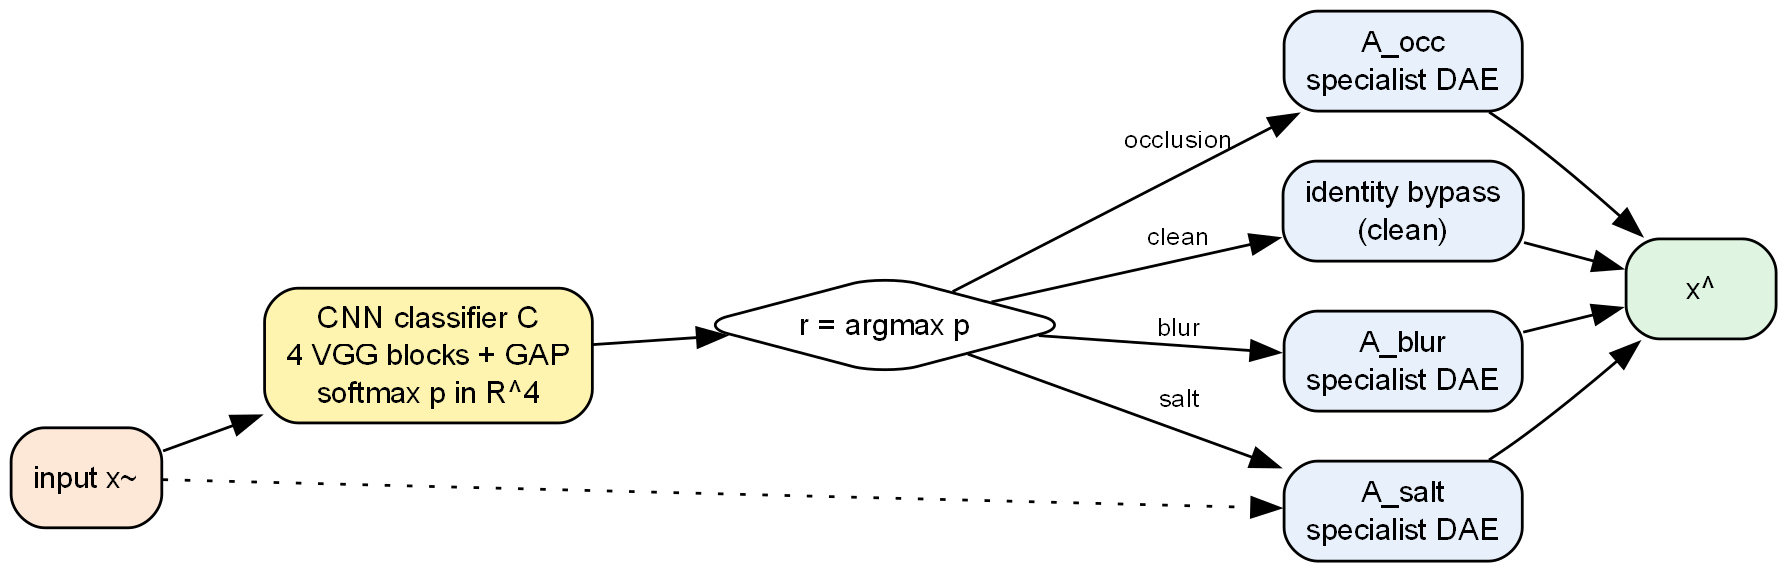
\includegraphics[width=\linewidth]{t2_hard.png}\caption{Hard routing.}\label{fig:t2arch}\end{figure}
\textbf{T2-RESULTS}

\section{Task 3: Jointly Trained Soft Mixture-of-Experts}
The gate $G$ shares the classifier architecture and weights; the experts are the three specialists plus an identity branch (Fig.~\ref{fig:t3arch}): $w=\mathrm{softmax}(G(\tilde x)/\tau)$, $\hat x=w_0\tilde x+\sum_{k=1}^3 w_kA_k(\tilde x)$. Training: (1) warm-up with experts frozen, only $G$ trained (lr $10^{-3}$); (2) joint fine-tuning of all parameters with a smaller learning rate. Specialist BatchNorm statistics are kept frozen during fine-tuning, a standard precaution when fine-tuning pretrained networks on a shifted input mixture. The loss is $\lambda_1\mathcal L_1+\lambda_s(1-\mathrm{SSIM})+\lambda_c\mathcal L_{CE}+\lambda_b\sum_k(\bar w_k-\frac14)^2$, where $\bar w_k$ is the batch-mean weight. Because our batches are exactly class-balanced, a uniform \emph{average} routing is the correct target, while individual images can still be routed sharply (a property that per-sample entropy penalties would destroy); this mirrors the load-balancing losses of~\cite{shazeer2017,fedus2022}. Optuna (8 trials, 1 warm-up + 3 joint epochs) tuned the joint lr, $\tau\in[0.5,2]$, $\lambda_c$, $\lambda_b$ and $\lambda_1$ (with $\lambda_s=1-\lambda_1$). Trials were pruned on median performance \emph{or} routing collapse (any branch with mean validation weight $<2\%$).
\begin{figure}[t]\centering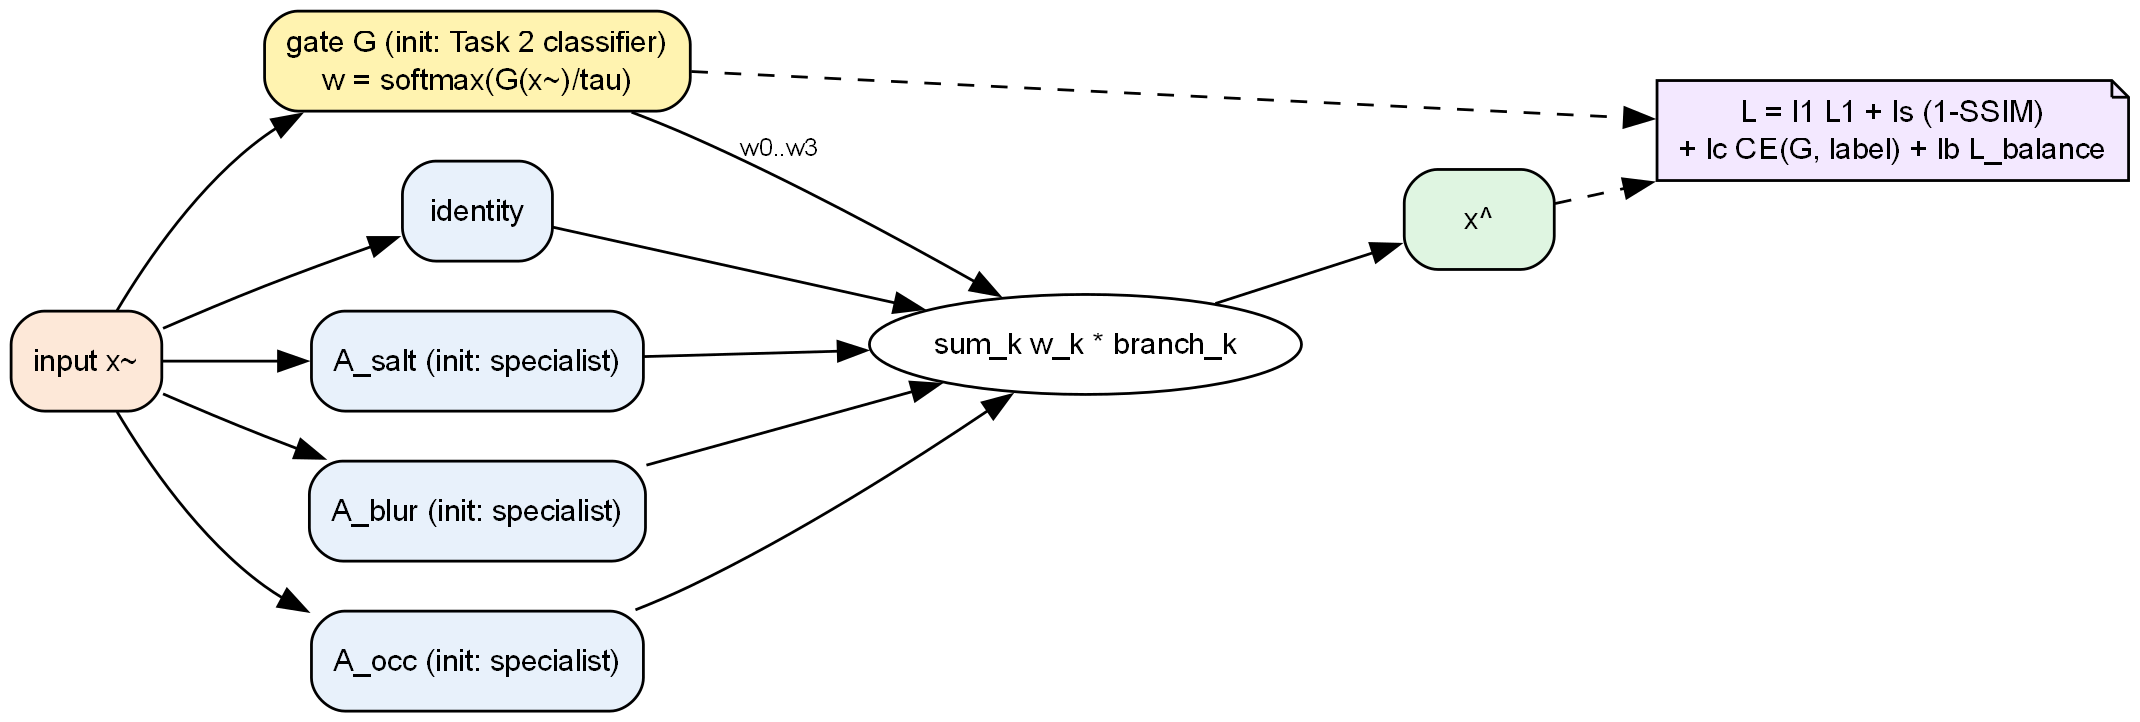
\includegraphics[width=\linewidth]{t3_moe.png}\caption{Soft MoE with identity branch.}\label{fig:t3arch}\end{figure}
\textbf{T3-RESULTS}

\section{Task 4: Style-Conditioned Face-to-Sketch cGAN}
FS2K's official train/test definitions are used; 15\% of the training portion (stratified by style, seed 42) forms the validation set, and the test set is never used for training or model selection. Photos (RGB) and sketches (grayscale) are resized to $128\times128$ and kept paired by name. Augmentation (random horizontal flip and an 8-pixel reflect-pad random crop) is drawn \emph{once} per pair and applied identically to photo and sketch, preserving pixel correspondence.
The generator (Fig.~\ref{fig:t4arch}) is a U-Net (6 down-sampling blocks to $2\times2$, 5 up-sampling blocks with skips, dropout in the first three decoder blocks, tanh output). A learned \texttt{nn.Embedding}(3,$E$) conditions both networks: in $G$ it is tiled and concatenated to the photo and also projected and added at the bottleneck; in the PatchGAN $D$ ($14\times14$ logits for $128^2$ inputs) it is tiled and concatenated to the photo--sketch pair. Losses: $\mathcal L_D=\frac12[\mathrm{BCE}(D(x,y,s),1)+\mathrm{BCE}(D(x,G(x,s),s),0)]$, $\mathcal L_G=\mathrm{BCE}(D(x,G(x,s),s),1)+\lambda_{L1}\|y-G(x,s)\|_1$; Adam$(0.5,0.999)$ with the pix2pix schedule (constant, then linear decay). The D-real, D-fake, G-adversarial and G-L1 losses and validation SSIM/L1 are logged separately, and the same 8 validation photos are rendered every 5 epochs. Optuna (15-epoch trials) tuned both learning rates, batch, base channels, dropout, embedding size and $\lambda_{L1}\in[10,200]$; the selected configuration was retrained for the full schedule. Because pixel metrics favour blurry outputs, the \emph{final} generator (end of LR decay) is deployed, not the epoch with the best validation SSIM.
\begin{figure}[t]\centering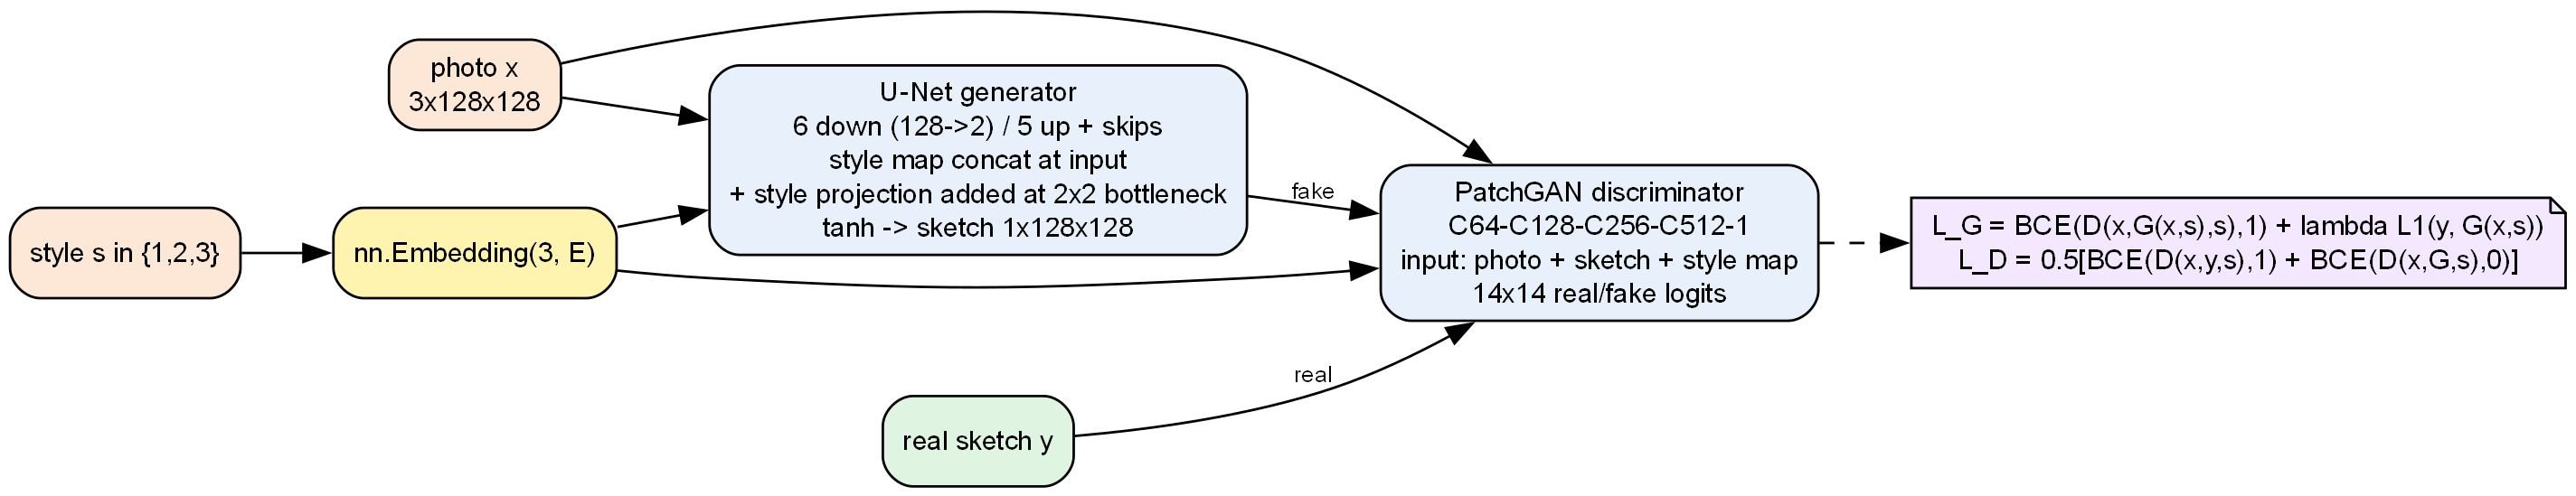
\includegraphics[width=\linewidth]{t4_cgan.png}\caption{Style-conditioned cGAN.}\label{fig:t4arch}\end{figure}
\textbf{T4-RESULTS}

\section{Application Design and Deployment}
The interface was first designed in Google Stitch (Fig.~\ref{fig:stitch}) and implemented in React + Tailwind CSS (Fig.~\ref{fig:app}): a sidebar with the four required workspaces (Universal Restoration, Hard-Routed Restoration, Soft Mixture-of-Experts Restoration, Face-to-Sketch Generator) and a System page. Each restoration workspace lets the user upload an image or pick a sample, optionally apply a runtime corruption with test-set severities and a seed, and shows the clean reference, model input, output and error map together with PSNR/L1, inference time per stage, classifier probabilities with the selected expert, or the four MoE weights as bars and a stacked contribution strip. The sketch workspace supports upload or webcam capture, three styles, side-by-side display and download. The FastAPI backend validates type and size (415/413/422 errors), decodes with EXIF correction, resizes exactly as in training, runs ONNX Runtime and returns base64 PNGs plus JSON metadata (Fig.~\ref{fig:apparch}). It exposes \texttt{/api/health}, \texttt{/api/info}, \texttt{/api/restore/\{universal,hard,soft\}}, \texttt{/api/sketch} and \texttt{/api/corrupt}. Frontend (nginx) and backend run in separate containers; \texttt{docker compose up --build} starts everything, and the models are mounted read-only from \texttt{models\_onnx/}.
\begin{figure}[t]\centering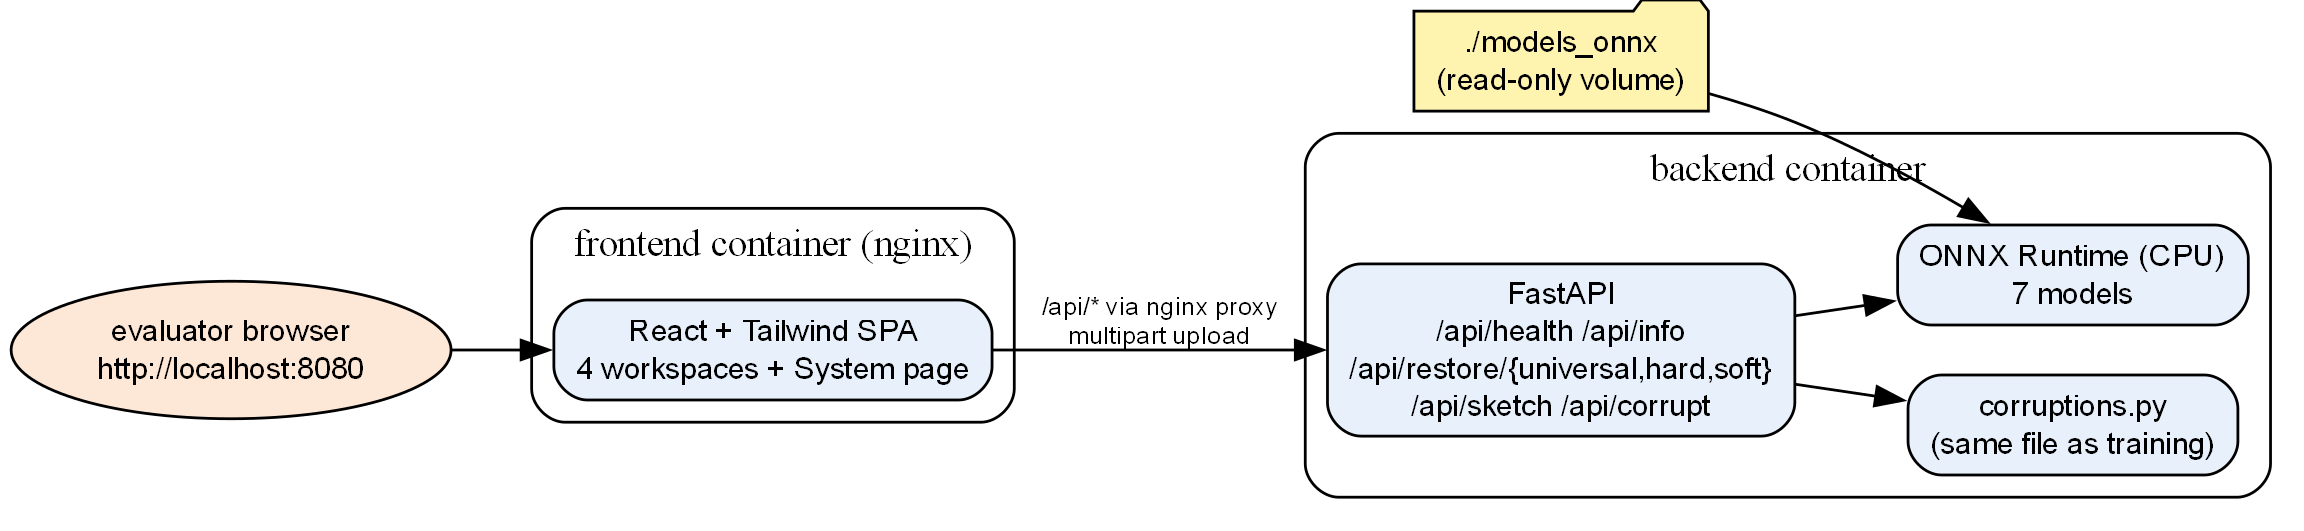
\includegraphics[width=\linewidth]{app.png}\caption{Deployment architecture.}\label{fig:apparch}\end{figure}
\textbf{APP-FIGURES}

\section{Limitations}
\textbf{LIMITATIONS}

\section{Conclusion}
\textbf{CONCLUSION}

\appendices
\section{AI-Use Statement}
\textbf{AI-USE}

\bibliographystyle{IEEEtran}
\begin{thebibliography}{99}
\bibitem{vincent2008} P.~Vincent, H.~Larochelle, Y.~Bengio and P.-A.~Manzagol, ``Extracting and composing robust features with denoising autoencoders,'' in \emph{Proc. ICML}, 2008.
\bibitem{mao2016} X.-J.~Mao, C.~Shen and Y.-B.~Yang, ``Image restoration using very deep convolutional encoder-decoder networks with symmetric skip connections,'' in \emph{Proc. NeurIPS}, 2016.
\bibitem{zhao2017} H.~Zhao, O.~Gallo, I.~Frosio and J.~Kautz, ``Loss functions for image restoration with neural networks,'' \emph{IEEE Trans. Comput. Imaging}, vol.~3, no.~1, 2017.
\bibitem{jacobs1991} R.~A.~Jacobs, M.~I.~Jordan, S.~J.~Nowlan and G.~E.~Hinton, ``Adaptive mixtures of local experts,'' \emph{Neural Computation}, vol.~3, no.~1, 1991.
\bibitem{shazeer2017} N.~Shazeer \emph{et al.}, ``Outrageously large neural networks: The sparsely-gated mixture-of-experts layer,'' in \emph{Proc. ICLR}, 2017.
\bibitem{fedus2022} W.~Fedus, B.~Zoph and N.~Shazeer, ``Switch Transformers: Scaling to trillion parameter models with simple and efficient sparsity,'' \emph{JMLR}, vol.~23, 2022.
\bibitem{isola2017} P.~Isola, J.-Y.~Zhu, T.~Zhou and A.~A.~Efros, ``Image-to-image translation with conditional adversarial networks,'' in \emph{Proc. CVPR}, 2017.
\bibitem{mirza2014} M.~Mirza and S.~Osindero, ``Conditional generative adversarial nets,'' arXiv:1411.1784, 2014.
\bibitem{miyato2018} T.~Miyato and M.~Koyama, ``cGANs with projection discriminator,'' in \emph{Proc. ICLR}, 2018.
\bibitem{fan2022} D.-P.~Fan \emph{et al.}, ``Facial-sketch synthesis: A new challenge,'' \emph{Machine Intelligence Research}, vol.~19, 2022.
\bibitem{akiba2019} T.~Akiba, S.~Sano, T.~Yanase, T.~Ohta and M.~Koyama, ``Optuna: A next-generation hyperparameter optimization framework,'' in \emph{Proc. KDD}, 2019.
\bibitem{parkhi2012} O.~M.~Parkhi, A.~Vedaldi, A.~Zisserman and C.~V.~Jawahar, ``Cats and dogs,'' in \emph{Proc. CVPR}, 2012.
\end{thebibliography}
\end{document}
